\documentclass[12pt]{article}
\usepackage{amsmath, amssymb, graphicx, tikz}
\usetikzlibrary{positioning}
\usepackage[margin=1in]{geometry}
\usepackage{physics}
\usepackage{float}
\usepackage{enumitem}
\usepackage{titling}
\DeclareMathOperator{\sinc}{sinc}
\setlength{\droptitle}{-2em}

\title{EE 115 – Homework 3 Solutions}
\author{Kaushik Vada}
\date{October 18, 2025}

\begin{document}
\maketitle

\section*{Problem 1}

---

\begin{enumerate}[label=(\alph*)]
\item The baseband spectrum is
\[
M(f) = \frac{1}{2}\,\mathrm{rect}\left(\frac{f}{2}\right),
\]
so \(M(f) = \frac{1}{2}\) for \(|f| < 1\) and \(0\) elsewhere, as shown in Fig.~\ref{fig:prob1a}.

\begin{figure}[H]
\centering
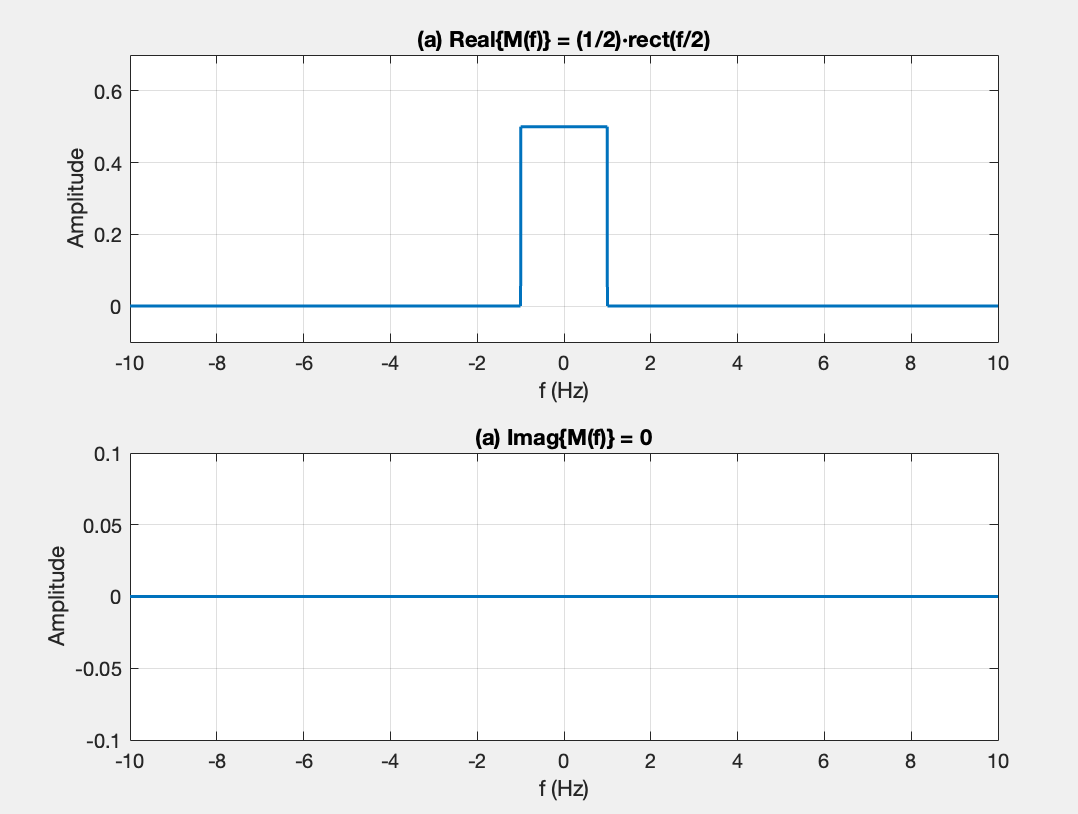
\includegraphics[width=0.55\textwidth]{images/Question1/1a.png}
\caption{Baseband spectrum of \(m(t)=\sinc(2t)\).}
\label{fig:prob1a}
\end{figure}

\item Multiplying by \(\cos(2\pi 5t)\) shifts the spectrum by \(\pm 5\):
\[
M_c(f) = \frac{1}{2}\left[ M(f-5) + M(f+5) \right],
\]
which produces two rectangular lobes centered at \( f = \pm 5 \), each of width \(2\) and amplitude \( \frac{1}{4} \). The full sketch is shown in Fig.~\ref{fig:prob1b}.

\begin{figure}[H]
\centering
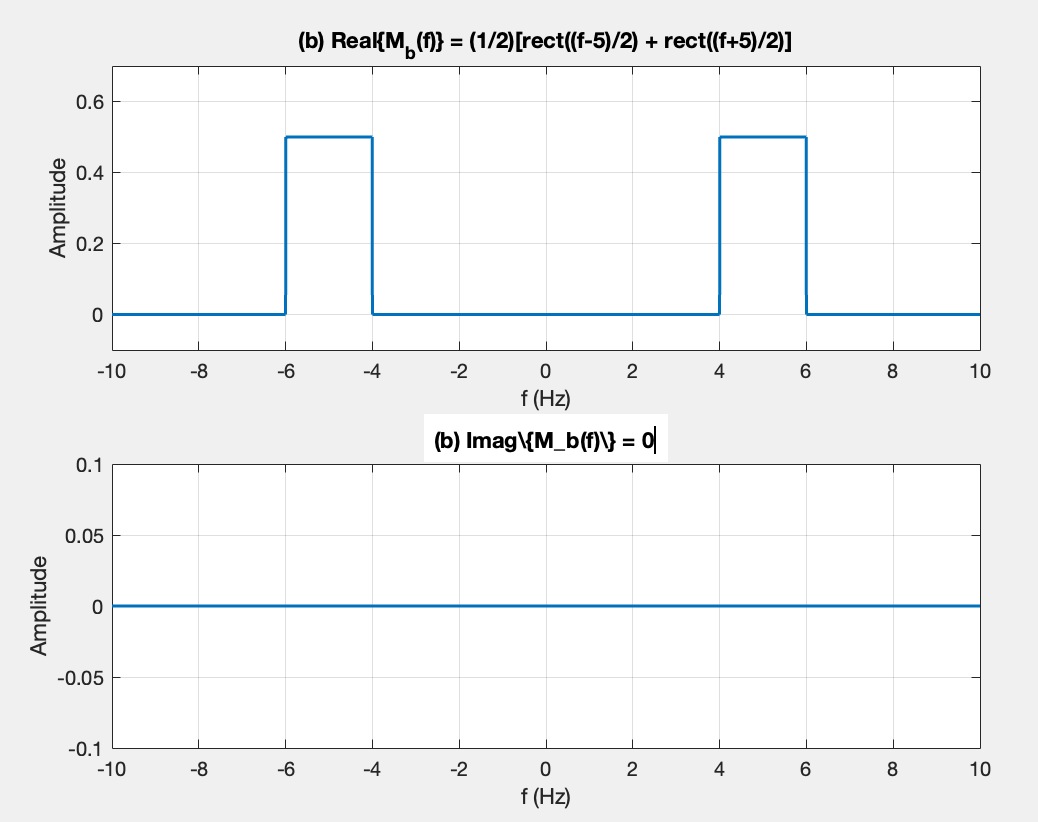
\includegraphics[width=0.55\textwidth]{images/Question1/1b.png}
\caption{Double-sideband spectrum of \(m(t)\cos(2\pi 5t)\).}
\label{fig:prob1b}
\end{figure}

\item Modulating by \(\sin(2\pi 5t)\) yields
\[
M_s(f) = \frac{1}{2j}\left[ M(f-5) - M(f+5) \right],
\]
so the real part is zero and the imaginary part is
\[
\Im\{M_s(f)\} = \frac{1}{2}\left[\mathrm{rect}\left(\frac{f-5}{2}\right) - \mathrm{rect}\left(\frac{f+5}{2}\right)\right],
\]
which is odd-symmetric as illustrated in Fig.~\ref{fig:prob1c}.

\begin{figure}[H]
\centering
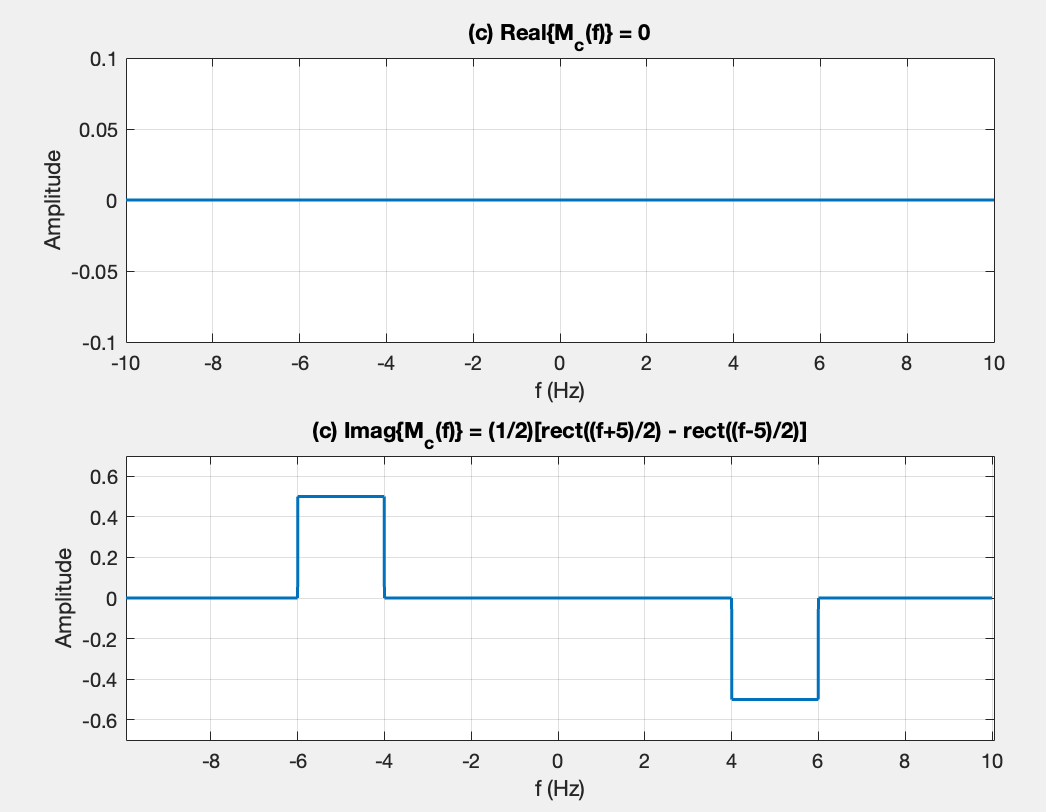
\includegraphics[width=0.55\textwidth]{images/Question1/1c.png}
\caption{Spectrum of \(m(t)\sin(2\pi 5t)\) highlighting the imaginary symmetry.}
\label{fig:prob1c}
\end{figure}
\end{enumerate}

---

\newpage

\section*{Problem 2 (30 points)}

Assume \(m(t) = 2\sinc(2t) = \dfrac{\sin(2\pi t)}{\pi t}\).

\begin{enumerate}[label=(\alph*)]
\item Determine its Hilbert transform \(\hat{m}(t)\). First find the spectrum:
\[
M(f) = 2 \cdot \frac{1}{2}\,\mathrm{rect}\!\left(\frac{f}{2}\right) = \mathrm{rect}\!\left(\frac{f}{2}\right),
\]
so \(M(f)=1\) for \(|f|<1\) and \(0\) otherwise. Applying the Hilbert multiplier gives
\[
\hat{M}(f) = -j\,\mathrm{sgn}(f)\,M(f) = 
\begin{cases}
-j, & 0 < f < 1, \\
+j, & -1 < f < 0, \\
0, & |f| \ge 1 .
\end{cases}
\]
The inverse transform is then
\begin{align*}
\hat{m}(t) &= \int_{-1}^{1} \hat{M}(f)\,e^{j2\pi ft}\,df \\
&= \int_{-1}^{0} j\,e^{j2\pi ft}\,df + \int_{0}^{1} (-j)\,e^{j2\pi ft}\,df \\
&= \frac{1}{2\pi t}\Big[1 - e^{-j2\pi t} + 1 - e^{j2\pi t}\Big] \\
&= \frac{1 - \cos(2\pi t)}{\pi t},
\end{align*}
with the \(t=0\) value obtained by continuity as \(\hat{m}(0)=0\).

\item The sketches of both \(M(f)\) and \(\hat{M}(f)\) over all frequencies are provided in Fig.~\ref{fig:prob2b}:

\begin{figure}[H]
\centering
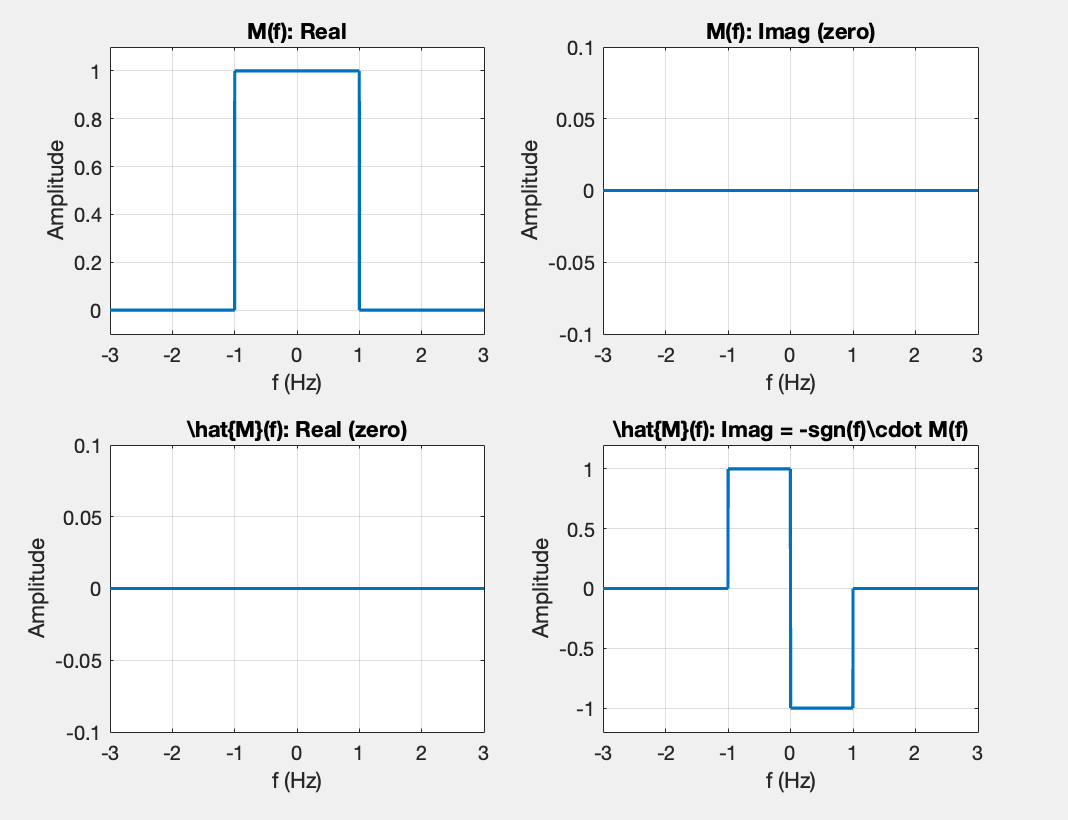
\includegraphics[width=0.55\textwidth]{images/Question2/2b.png}
\caption{Sketches of \(M(f)\) (blue) and \(\hat{M}(f)\) (green) for part (b).}
\label{fig:prob2b}
\end{figure}

\item The time-domain sketches of \(m(t)\) and \(\hat{m}(t)\) for all \(t\) are shown in Fig.~\ref{fig:prob2c}, highlighting the even/odd symmetry pair.

\begin{figure}[H]
\centering
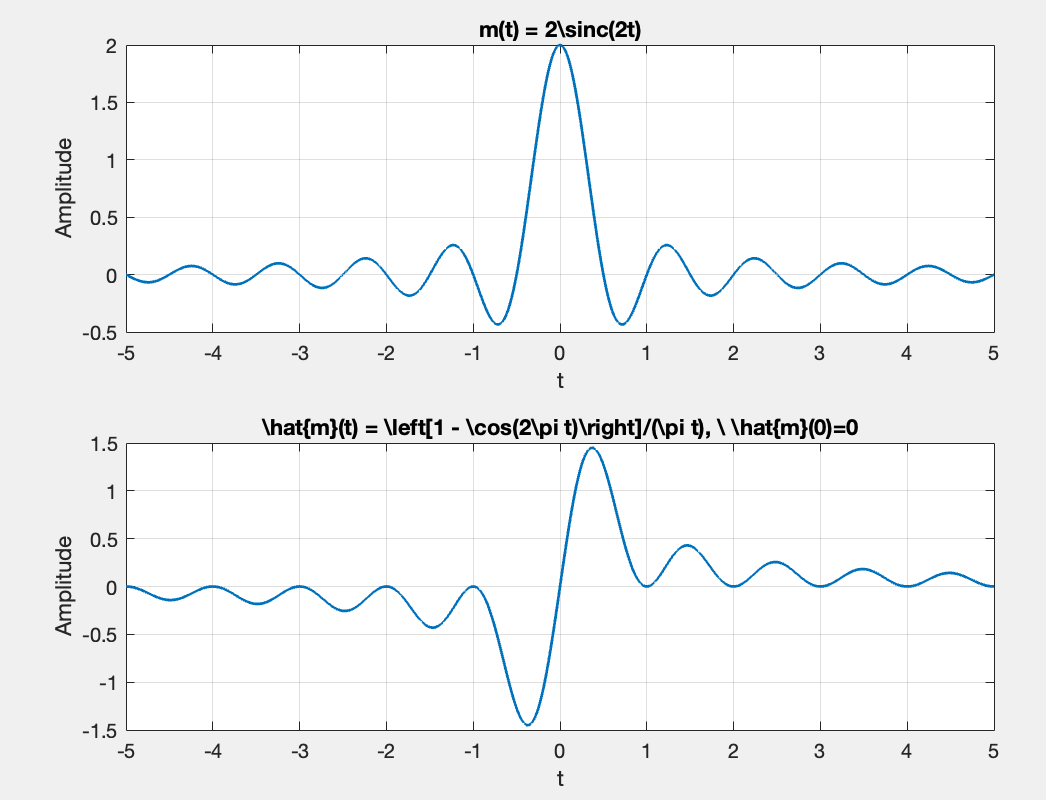
\includegraphics[width=0.55\textwidth]{images/Question2/2c.png}
\caption{Sketches of \(m(t)\) and its Hilbert transform \(\hat{m}(t)\) for part (c).}
\label{fig:prob2c}
\end{figure}
\end{enumerate}

---

\section*{Problem 3}

\textbf{Given: } 
\[
u(t) = a(t)\cos(2\pi f_c t) - b(t)\sin(2\pi f_c t)
\]

\textbf{Goal: } Recover \(a(t)\) and \(b(t)\) using coherent demodulation.

\begin{figure}[H]
\centering
\begin{tikzpicture}[scale=1.1, node distance=1.2cm]
\node (u) {$u(t)$};
\node[below left=of u] (mix1) {$\times \cos(2\pi f_c t)$};
\node[below right=of u] (mix2) {$\times \sin(2\pi f_c t)$};
\node[below=of mix1] (LPF1) [draw, rectangle, minimum width=2cm, minimum height=0.8cm] {LPF};
\node[below=of mix2] (LPF2) [draw, rectangle, minimum width=2cm, minimum height=0.8cm] {LPF};
\node[below=of LPF1] (aout) {$a(t)$};
\node[below=of LPF2] (bout) {$b(t)$};

\draw[->] (u) -- (mix1);
\draw[->] (u) -- (mix2);
\draw[->] (mix1) -- (LPF1);
\draw[->] (mix2) -- (LPF2);
\draw[->] (LPF1) -- (aout);
\draw[->] (LPF2) -- (bout);
\end{tikzpicture}
\caption*{Coherent Demodulation Block Diagram}
\end{figure}

\end{document}
